\section{Dados e análise exploratória}
O MovieLens 100k \cite{movielens} reúne 100.000 notas de 1 a 5, atribuídas por 943 usuários a
1.682 filmes. Os arquivos originais foram preservados: não há notas ausentes nos registros, valores fora
de $[1,5]$ ou pares usuário--filme duplicados. Não houve exclusão nem imputação;
posições sem avaliação permanecem ausentes.

A média é 3,53 e 55,4\% das avaliações são
4 ou 5. As distribuições de atividade, porém, são bastante assimétricas
(Figura~\ref{fig:eda}).

\begin{figure}[H]
\centering
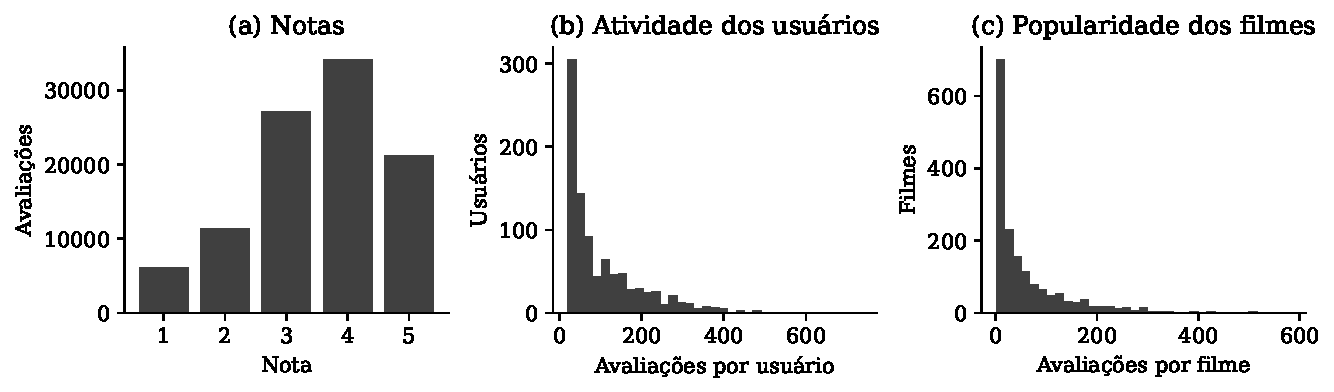
\includegraphics[width=\textwidth]{figuras/ativ_eda.pdf}
\caption{Distribuição das notas e da quantidade de avaliações por usuário e
por filme. As caudas à direita mostram a concentração da atividade.}
\label{fig:eda}
\end{figure}

\begin{table}[H]
\centering\small
\caption{Quantidade de avaliações. A distância entre média e mediana destaca
a assimetria observada nos histogramas.}
\begin{tabular}{@{}lrrrrr@{}}
\toprule
Unidade & Média & Mínimo & Mediana & 3º quartil & Máximo\\
\midrule
Usuário & 106,0 & 20 & 65 & 148 & 737\\
Filme & 59,5 & 1 & 27 & 80 & 583\\
\bottomrule
\end{tabular}
\end{table}

A matriz tem 93,70\% de posições sem nota, e metade das avaliações se concentra
em 12,78\% do catálogo. No outro extremo, 384 filmes têm até cinco avaliações,
dos quais 141 têm apenas uma. Assim, notas médias extremas podem ter pouco
suporte, e nem sempre há muitos filmes em comum para comparar dois usuários.

Os dados descrevem avaliações observadas, não o gosto por todos os filmes
não avaliados. A coleta ocorreu em 1997--1998; 71,0\% dos usuários cadastrados
são homens e a mediana de idade é 31 anos. Os dados demográficos não entram no treinamento.
